\documentclass{sig-alternate}
\usepackage{amssymb}
\setcounter{tocdepth}{3}
\usepackage{listings}
\usepackage{booktabs}
\usepackage{mathtools}
\usepackage{tabularx}
\usepackage{fixltx2e}
\PassOptionsToPackage{hyphens}{url}\usepackage{hyperref}
\usepackage[hyphens]{url}
\usepackage{upquote,textcomp}
\lstset{breaklines=true, basicstyle=\scriptsize\ttfamily, upquote=true}

\usepackage{fancyvrb}
\VerbatimFootnotes
\usepackage{cprotect}

\usepackage{graphicx}
\makeatletter
\def\maxwidth#1{\ifdim\Gin@nat@width>#1 #1\else\Gin@nat@width\fi}
\makeatother

\usepackage{amsmath}
\usepackage{pmml-new}

\usepackage{color,graphics,array,csscolor}

\usepackage{fontspec,unicode-math}
\usepackage[Latin,Greek]{ucharclasses}
\setTransitionsForGreek{\fontspec{Times New Roman}}{}



\makeatletter
\let\@copyrightspace\relax
\makeatother
\begin{document}
\title{TANKER: Distributed Architecture for Named Entity Recognition and Disambiguation}

\numberofauthors{4}
\author{
\alignauthor
Sandro A. Coelho\\
\affaddr{InfAI, University of Leipzig, Leipzig, Germany}\\
\email{sandro.coelho@ice.ufjf.br}
\alignauthor
Diego Moussalem\\
\affaddr{AKSW, University of Leipzig, Leipzig, Germany}\\
\email{moussalem@informatik.uni-leipzig.de}
\alignauthor
Gustavo C. Publio\\
\affaddr{AKSW, University of Leipzig, Leipzig, Germany}\\
\email{publio@informatik.uni-leipzig.de}
\and
\alignauthor
Diego Esteves\\
\affaddr{SDA Research Group, University of Bonn, Bonn, Germany}\\
\email{esteves@cs.uni-bonn.de}}
\maketitle

\begin{abstract}
Named Entity Recognition and Disambiguation (NERD) systems have recently been widely researched to deal with the significant growth of the Web. NERD systems are crucial for several Natural Language Processing (NLP) tasks such as summarization, understanding, and machine translation. However, there is no standard interface specification, i.e. these systems may vary significantly either for exporting their outputs or for processing the inputs. Thus, when a given company desires to implement more than one NERD system, the process is quite exhaustive and prone to failure. In addition, industrial solutions demand critical requirements, e.g., large-scale processing, completeness, versatility, and licenses. Commonly, these requirements impose a limitation, making good NERD models to be ignored by companies. This paper presents TANKER, a distributed architecture which aims to overcome scalability, reliability and failure tolerance limitations related to industrial needs by combining NERD systems. To this end, TANKER relies on a micro-services oriented architecture, which enables agile development and delivery of complex enterprise applications. In addition, TANKER provides a standardized API which makes possible to combine several NERD systems at once.
\end{abstract}


\keywords{Entity Linking, Joining processes, Knowledge based systems, NER Architec-tures, Named Entity Recognition}

\begin{abstract}
We presented TANKER, a distributed architecture for combining NERD systems. In a preliminary overview, our approach can deal with a large-scale processing and a high number of requests. In addition, TANKER responds to the queries in an appropriate response time thus addressing the aforementioned gaps. As an immediate work, we intend to integrate more NERD systems in order to improve the fault tolerance and evaluate TANKER using GERBIL \cite{_Ref490775154} to see the real performance of it compared to other NERD systems. As a future work, we plan to include a KB management service for enabling TANKER to process different KBs altogether. Furthermore, in order to facilitate data management and follow best practices in terms of reproducibility of experiments, we will integrate TAKER within state of the art ML vocabularies and metadata repositories.
\end{abstract}


\keywords{Entity Linking, Joining processes, Knowledge based systems, NER Architec-tures, Named Entity Recognition}

\section{INTRODUCTION}

The Internet has been growing at an explosive rate for several years, which make harder to handle the big amount of information diffused in diverse formats, such as text, audio and, video. Currently, the Web produces more than 2.5 exabytes of data per day\footnote{\url{http://www.northeastern.edu/levelblog/2016/05/13/how-much-data-produced-every-day/}}. Therefore, the challenge of indexing, formatting, and making the information available to the users has arisen every day, which makes a critical scenario. In order to deal with such variety of contents, refined NLP techniques are required.

One of the most important NLP techniques is Named Entity Recognition and Disambiguation (NERD). The task aims at recognizing the entities and their types in raw texts and linking them to distinct Knowledge Base (KB)s \cite{_Ref490759706}. In addition, NERD systems enable the processing of unstructured texts to provide useful data for information retrieval, information extraction, machine translation, question answering systems and automatic summarization tools.

Although NERD approaches have been widely researched nowadays and shown good precision, they still present inefficient time-performance algorithms and poor versatility. In an industrial environment, a given newspaper company which desires to annotate their news can deal with different subjects in the same document. It makes the use of distinctive NERD systems and KBs harder. On the other hand, financial companies handle very large documents and the current NERD tools do not deliver the response in a reasonable time (e.g., they may take almost half day to deliver the results from a big data set\footnote{ See the average time in \url{http://gerbil.aksw.org/gerbil/experiment?id=201701260017}}). For instance, DBpedia Spotlight \cite{_Ref490759726} is able to process only 120 queries per minute\footnote{\url{https://github.com/dbpedia-spotlight/dbpedia-spotlight/wiki/User's-manual}} and also retrieves information only from DBpedia \cite{_Ref490759734}, which is not enough for enterprise companies who deal with large documents and different subjects. Therefore, the main lack is scalability which becomes a key factor for academic solutions to be adopted by the industrial environment.

Early efforts have focused on algorithms and evaluations, resulting in stand-alone applications that aimed to solve problems in specific domains. For example, Rizzo et al.  \cite{_Ref490759749} and Borodino et al.  \cite{_Ref490759761} proposed the combination of NERD systems for industrial solutions, but they did not focus on scalability. Thus, it becomes difficult to use them in real cases. Moreover, the systems must be checked whether there is any limitation for using in distributed environments regarding their licenses.

To this end, we present TANKER, an approach to address the aforementioned gaps by combining NERD solutions through a micro-services architecture. TANKER is a REST based service that decreases drawbacks especially with regards to integration, licensing, outdated technologies and availability/scalability. The main contributions intended with our work are:
\begin{itemize}
\item {\em Scalability}: TANKER allows to start new service instances by language/domain in response to rising demand with a round-robin distribution strategy.
\item {\em Fault tolerance}: using a client-side IPC library, a request can be handled for {\em N} configured available servers
\item {\em Completeness}: under the same request, TANKER can query one-to-many services to provide better results.
\end{itemize}

The paper is structured as follows: In the next section, we present the related works. Section Section~\ref{_Ref490760383} presents the TANKER architecture in details and explains how TANKER address the gaps pertaining to industrial solutions. In Section Section~\ref{_Ref490760402} we present the primary implementation of TANKER. Finally, we give an outlook on further directions and possibilities for TANKER in Section Abstract.

\section{RELATED WORK}

To the best of our knowledge, there is no work proposing a distributed architecture based on micro-services, especially focusing on its infrastructure and scalability. However, there are two works which had proposed distinct architectures for combining NERD systems without relying on machine learning (ML) algorithms. They are as follows:
\begin{itemize}
\item {\em NERD framework}: In 2012, proposed a generic framework which groups either commercial and research approaches among several entity recognition tools. The Named Entity Recognition (NER) tools are made available via Web APIs and they use a hybrid approach for presenting the different outputs of each NER tool via a unique response. Thus, providing users the opportunity to easily query each of these services through the same setup and compare their outputs. In addition, NERD is tailored for entity recognition of Twitter streams and has a public web API\footnote{\url{http://nerd.eurocom.fr}}. 
\item {\em HERMES framework}: The authors proposed a novel NLP framework dubbed HERMES which focuses on addressing the performance at the infrastructure layer. HERMES provides an Entity Recognition and Disambiguation service, enhanced with three features (topic extraction, topic labeling and topic explanation). It uses Apache Kafka\footnote{\url{http://kafka.apache.org}}to deal with message queues. However, their implementation comprises of asynchronous modules which does not consider the response time. This implies several challenges for developers, as it is hard to deal with different kinds of failure in asynchronous scenarios. Although Hermes architecture is based on modules, there is no web service or API provided by this solution.
\end{itemize}

In terms of components, i.e. NER, Entity Linking (EL) and NERD models, there are a plenty of available tools that could be integrated in our architecture. However, for the sake of space, we only introduce the approaches which are included in TANKER.
\begin{itemize}
\item {\em NER - Stanford NER}{\em \footnote{\url{https://nlp.stanford.edu/software/CRF-NER.shtml}}}{\em } \cite{_Ref490760481}is a Java implementation of a NER system. It labels sequences of words in a text which are the names of things, such as person and company names, or gene and protein names. It comes with well-engineered feature extractors for Named Entity Recognition, and many options for defining feature extractors. Stanford NER implements Conditional Random Fields (CRF) sequence models to perform NER tasks in pre-existing training sets, and one can also train a new model.
\item {\em NED -- AGDISTIS}{\em \footnote{\url{http://aksw.org/Projects/AGDISTIS.html}}}{\em } \cite{_Ref490760498}is an open source named entity disambiguation framework. Its early version can link entities by combining the HITS algorithm with label expansion strategies and string similarity measures. The newer version of it includes a new algorithm called MAG \cite{_Ref490760509}. MAG is a multilingual and deterministic algorithm which disambiguates entities from a given knowledge base by using HITS and PageRank along with an in-depth context search based on TF-IDF statistics. Based on this combination, it can efficiently detect the correct URIs for a given set of named entities within an input text. Furthermore, AGDISTIS is agnostic of the underlying knowledge base.
\item {\em NERD} - One of the first semantic approaches published in 2011, {\em DBpedia Spotlight}\footnote{\url{http://www.dbpedia-spotlight.org}} \cite{_Ref490759726} is a tool which combines NER and NED approaches for automatically annotating mentions of DBpedia resources \cite{_Ref490760525} in texts. In addition, Spotlight contains programmatic interfaces based on a vector-space representation of entities and cosine similarity for phrase spotting, i.e., recognition of phrases to be annotated. Moreover, it can export the results in various output formats such as XML, JSON/JSON-LD, RDF, NIF, and N3.
\end{itemize}

\section{ARCHITECTURE}\label{_Ref490760383}

TANKER was designed with portability and efficiency in mind. It was also designed to be customizable and extensible w.r.t. its user interface, functionality and the integration of underlying components. The overall architecture of TANKER is shown in TANKER is built using a microservice architecture  \cite{_Ref490760546}. Microservices have been getting a lot of attention and popularity in the recent years\footnote{\url{https://www.oreilly.com/ideas/the-evolution-of-scalable-microservices}} because of its significant benefits, especially w.r.t enabling the agile development, improving scalability, reliability and failure tolerance.

TANKER does not depend on any specific NERD service and is generic enough to be connected to any replacement microservice that abides by given service specification. This allows for simple configuration as well as adds a way to extend the functionality of the system - by adding or removing the microservices we can easily tailor the final user experience.

Additionally, microservices enforces a modularity level which is much faster to develop, and easier to understand and maintain. This architecture enables the development of each server independently by letting the architects free to choose appropriate technologies for different kind of problems. Thus, being possible to combine different programming languages in one single solution. The other components of TANKER are described in the sequence.
\begin{figure}[h!]
\centering
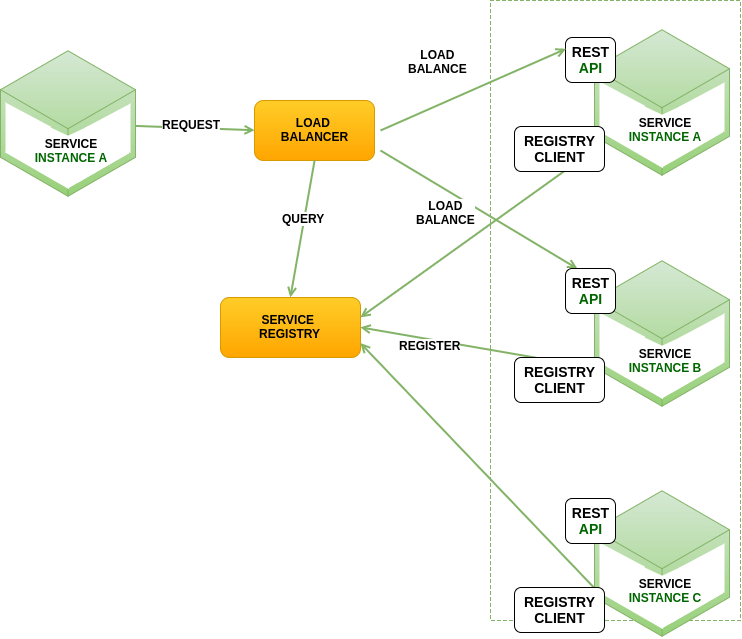
\includegraphics[width=\maxwidth{\columnwidth}]{./img/image1.png}
\cprotect\caption{Overview of TANKER architecture}
\label{_Ref490756012}
\end{figure}


\subsection{Scalability and Fault tolerance}

Scalability is the capability to handle a growing amount of processes within a computational system in a graceful manner, providing minimal interruptions to ongoing operations. This feature is mandatory for enterprise systems in addition to fault-tolerance, scaling up mode and some others, to deliver a good user experience at a minimum cost.

Most of NERD solutions are usually developed under synchronous or asynchronous requests. Both requests wait for a response, however, the synchronous might block the user interaction while the asynchronous does not. Commonly, distributed applications consider services interactions to decide which one will be used in its ecosystem. For instance, in synchronous requests, HTTP REST or Thrift\footnote{\url{https://thrift.apache.org/}}are adopted, on the other hand, the Advanced Message Queuing Protocol\footnote{\url{https://www.amqp.org/}}is used for asynchronous.

These request types infer on Inter-Process Communication (IPC) mechanisms. IPC software is a central piece of the architecture to ensure that microservices will scale and have fault-tolerance. This component is usually designed to be highly configurable and supports running in hybrid environments that are multi-region and multi-zone. To this end, TANKER supports synchronous interactions relying on Ribbon framework\footnote{\url{https://github.com/Netflix/ribbon}}as our IPC. Ribbon framework offers client-side software load balancing algorithms and a good set of configuration options such as connection timeouts and retry algorithms that fills in our requirements for NERD environments.

\subsection{Configuration}

The configuration of TANKER aims to reduce the complexity of management processes by using cloud services. Therefore, TANKER is based on Spring Cloud Config\footnote{\url{http://cloud.spring.io/spring-cloud-static/spring-cloud.html}} which offers a client-side application for exposing configuration of a distributed system. It is integrated with Spring ecosystem, but it can also be used with any application running in any programming language. This service uses the human-readable data serialization language (YAML\footnote{\url{http://yaml.org/}}), a widely spread format to describe services parameters and exposes all of them under a REST/API (see Listing 1